\chapter{ФОРМИРОВАНИЕ ДАТАСЕТА И ФИЗИЧЕСКИЕ ПРОВЕРКИ}

\section{Прямоугольный benchmark}
\todo{Описать прямоугольный quantum dot только как validation/control benchmark.}

\section{Датасет суперэллиптических квантовых точек с фиксированными n}
\todo{Dataset has 140 samples.}
\todo{$n$ values: 1.2, 2.0, 3.0, 4.0.}
\todo{$a$ values: 24, 27, 30, 33, 36.}
\todo{\texttt{aspect\_ratio} values: 0.67, 0.72, 0.78, 0.83, 0.89, 0.94, 1.0.}

\section{Проверка масштабирования $(E_0 + 4)a^2$}
\todo{Physical sanity checks: $(E_0 + 4)a^2$ stable within about 0.23\% to 1.31\% depending on $n$.}

\begin{figure}[htbp]
  \centering
  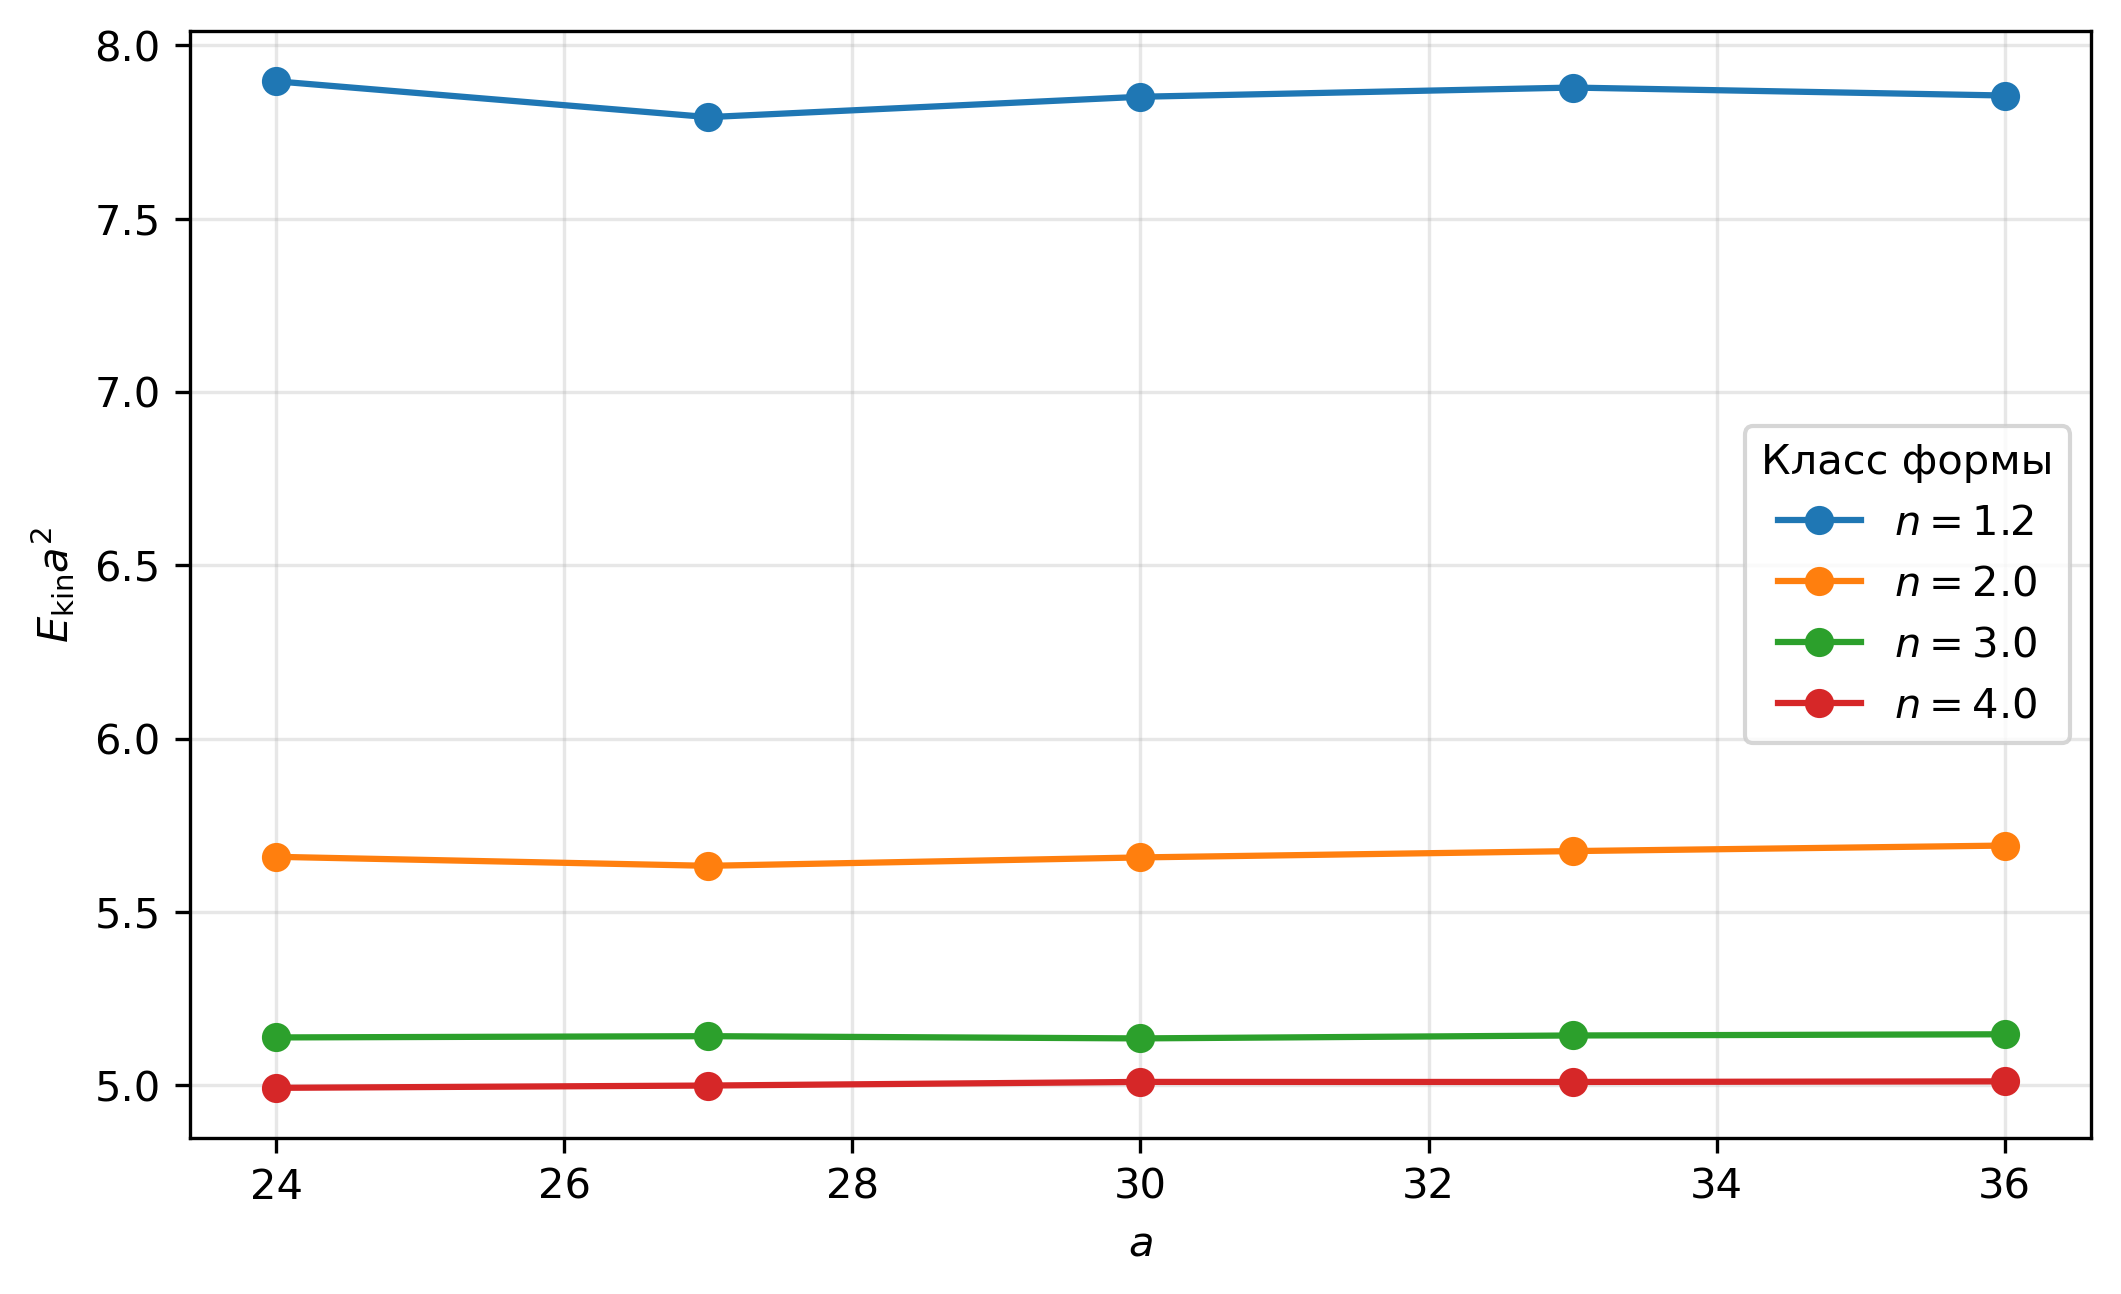
\includegraphics[width=0.85\textwidth]{../reports/assets/e0_kin_a2_scaling_by_n.png}
  \caption{TODO: Проверка масштабирования $(E_0 + 4)a^2$ для фиксированных $n$.}
\end{figure}

\section{Bessel sanity check для n = 2, aspect ratio = 1}
\todo{Bessel check at $a=36$ has about 2.03\% relative error.}

\begin{figure}[htbp]
  \centering
  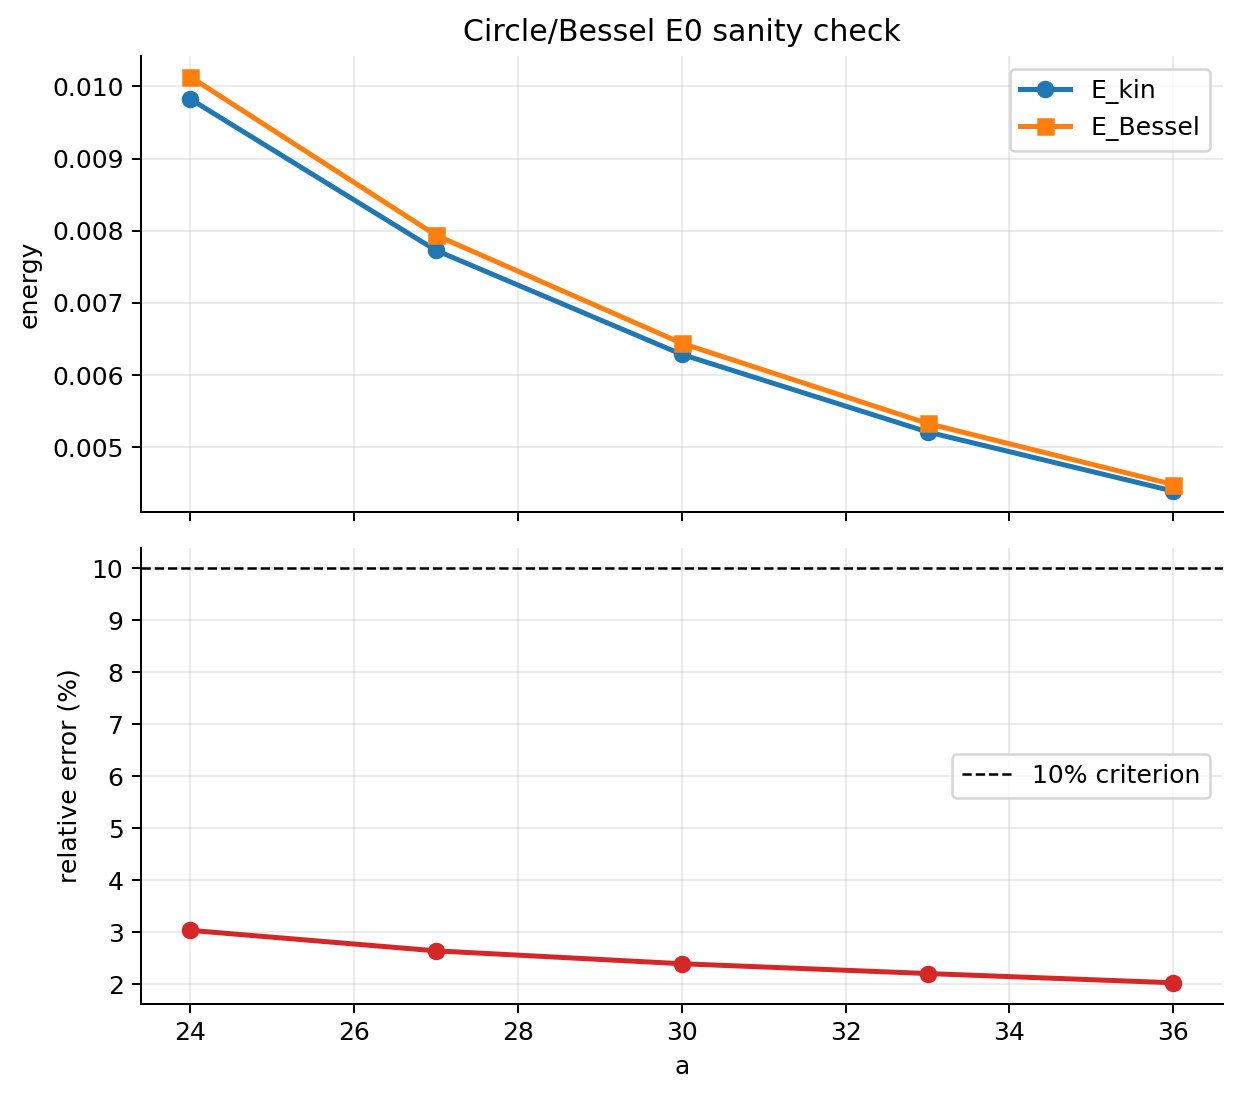
\includegraphics[width=0.85\textwidth]{../reports/assets/circle_bessel_e0_check.png}
  \caption{TODO: Bessel sanity check для кругового случая $n=2$, aspect ratio = 1.}
\end{figure}

\section{Вырождение уровней и исключение dE2 из основных целей}
\todo{$dE_2$ for $n=2$, aspect ratio = 1 is numerically zero across the inspected slice.}
\todo{Объяснить, почему это поддерживает diagnostic-only статус $dE_2$.}

\begin{figure}[htbp]
  \centering
  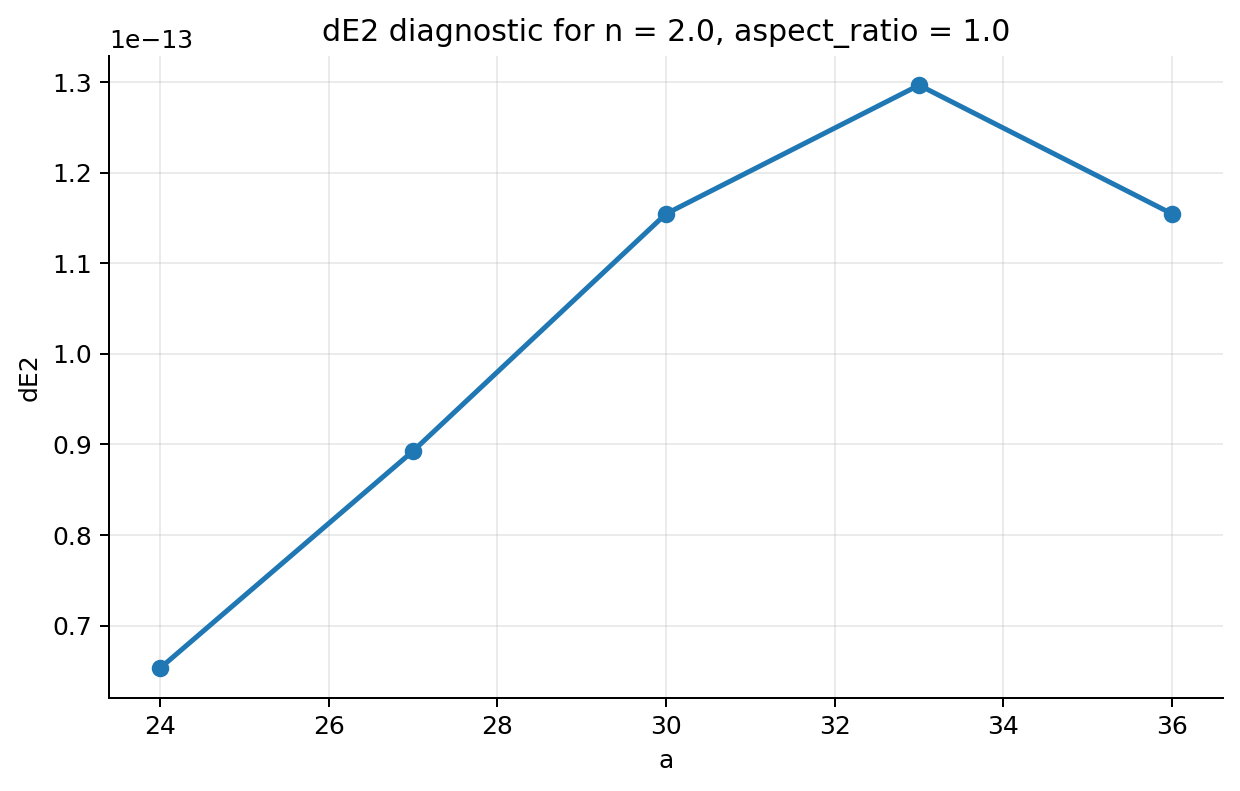
\includegraphics[width=0.80\textwidth]{../reports/assets/de2_near_degeneracy_n2_ar1.png}
  \caption{TODO: Диагностика near-degeneracy для $dE_2$ в круговом случае.}
\end{figure}

\section{Диагностики дискретизации границы}
\todo{$N_{\mathrm{sites}} / \mathrm{analytic\_area}$ ranges approximately from 0.98094 to 1.00761.}
\todo{max sublattice imbalance ratio about 2.16\%, largest at $n=1.2$, $a=24$, aspect ratio = 1.0.}

\begin{figure}[htbp]
  \centering
  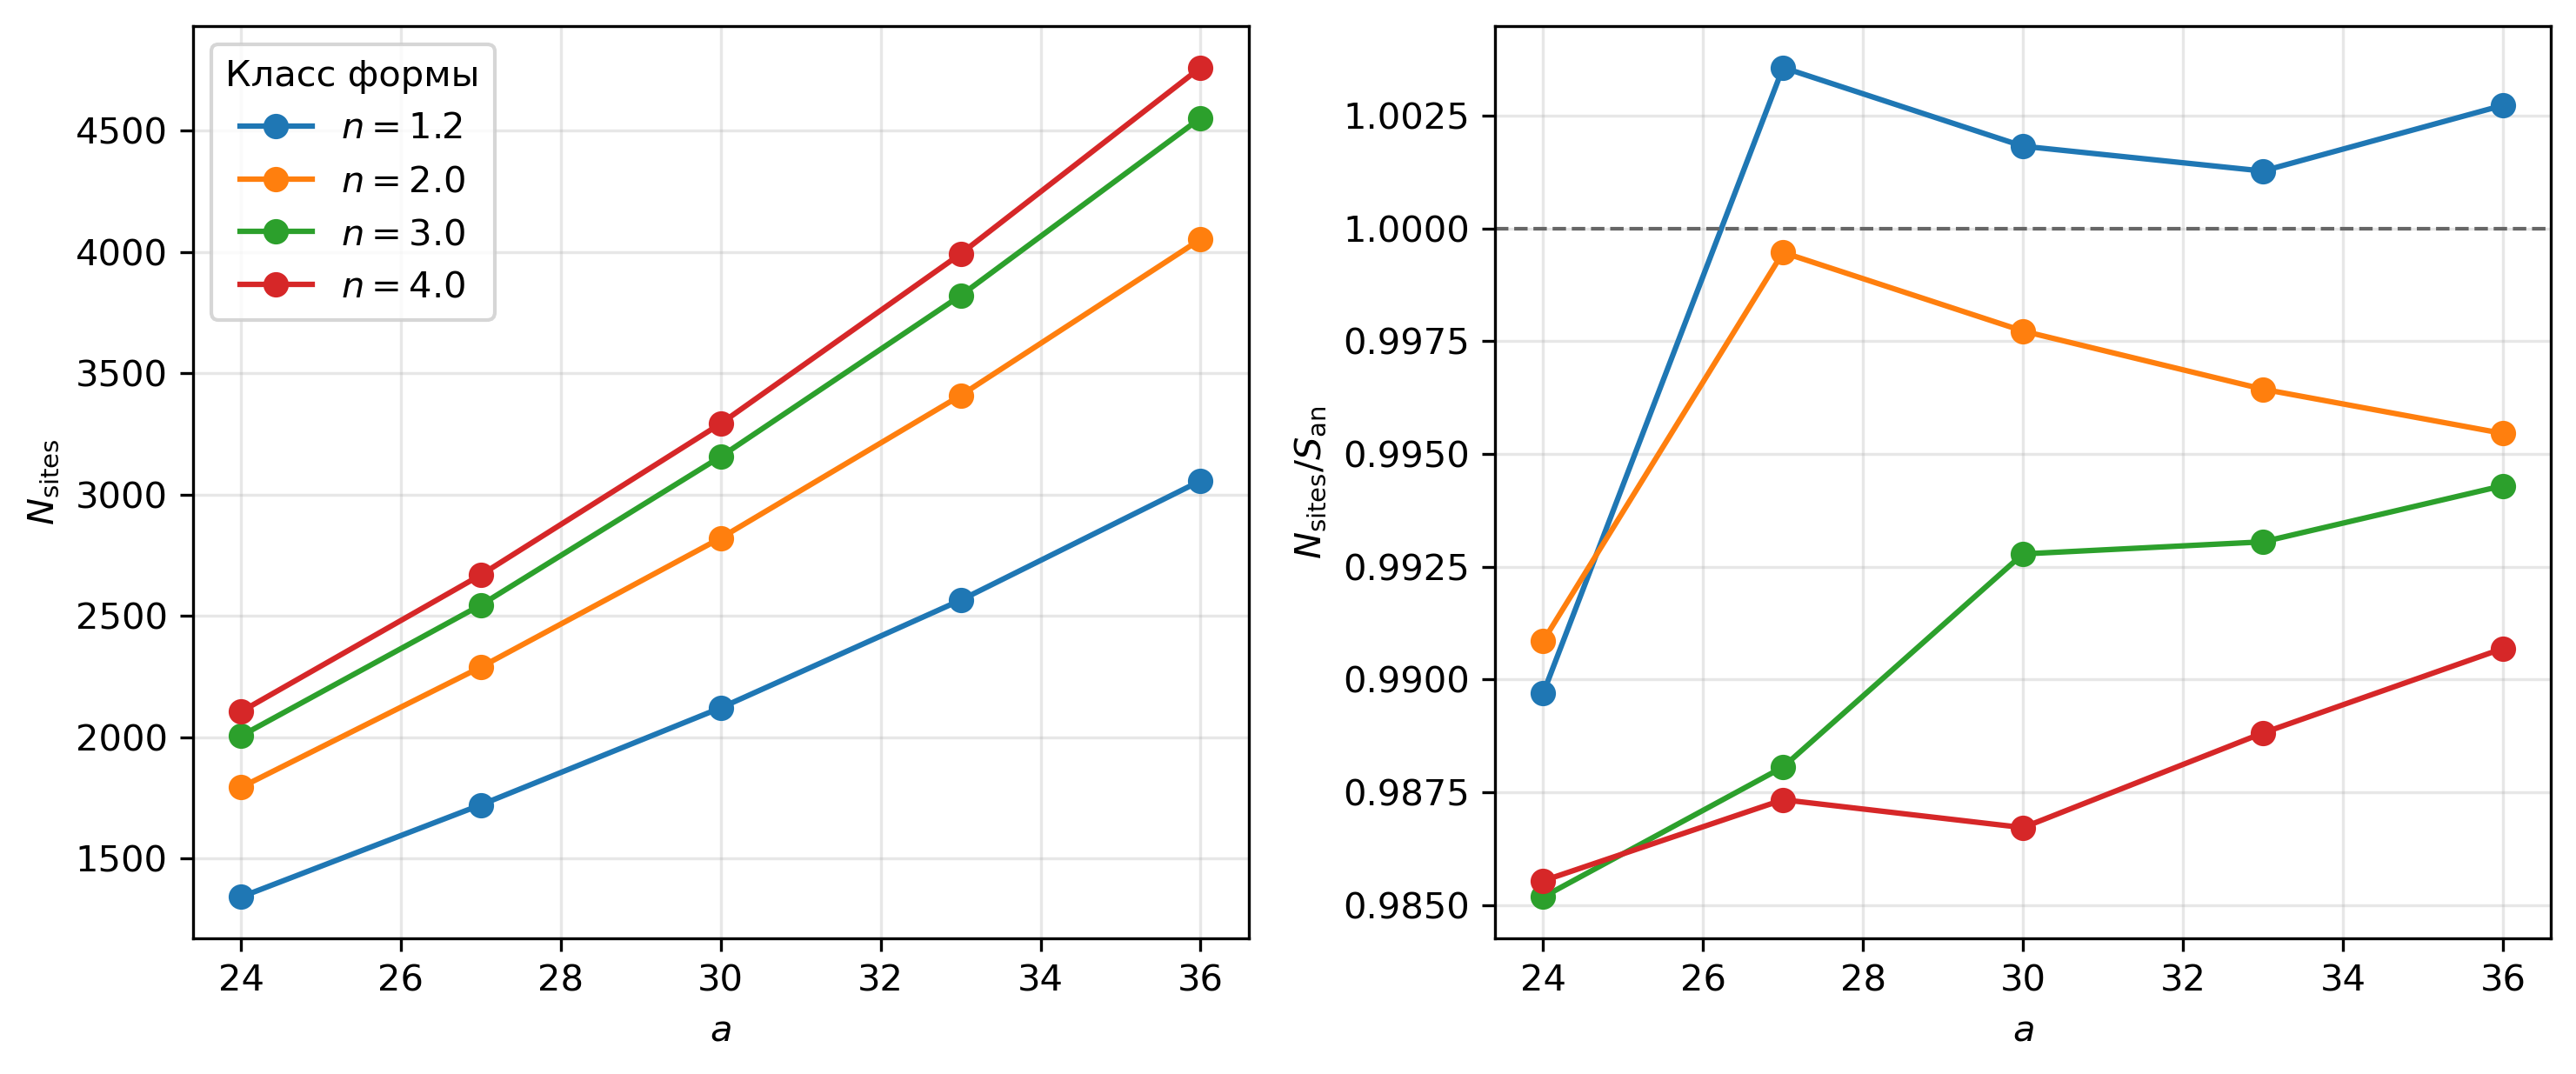
\includegraphics[width=0.85\textwidth]{../reports/assets/nsites_area_ratio_by_n.png}
  \caption{TODO: Сравнение числа узлов и аналитической площади.}
\end{figure}

\begin{figure}[htbp]
  \centering
  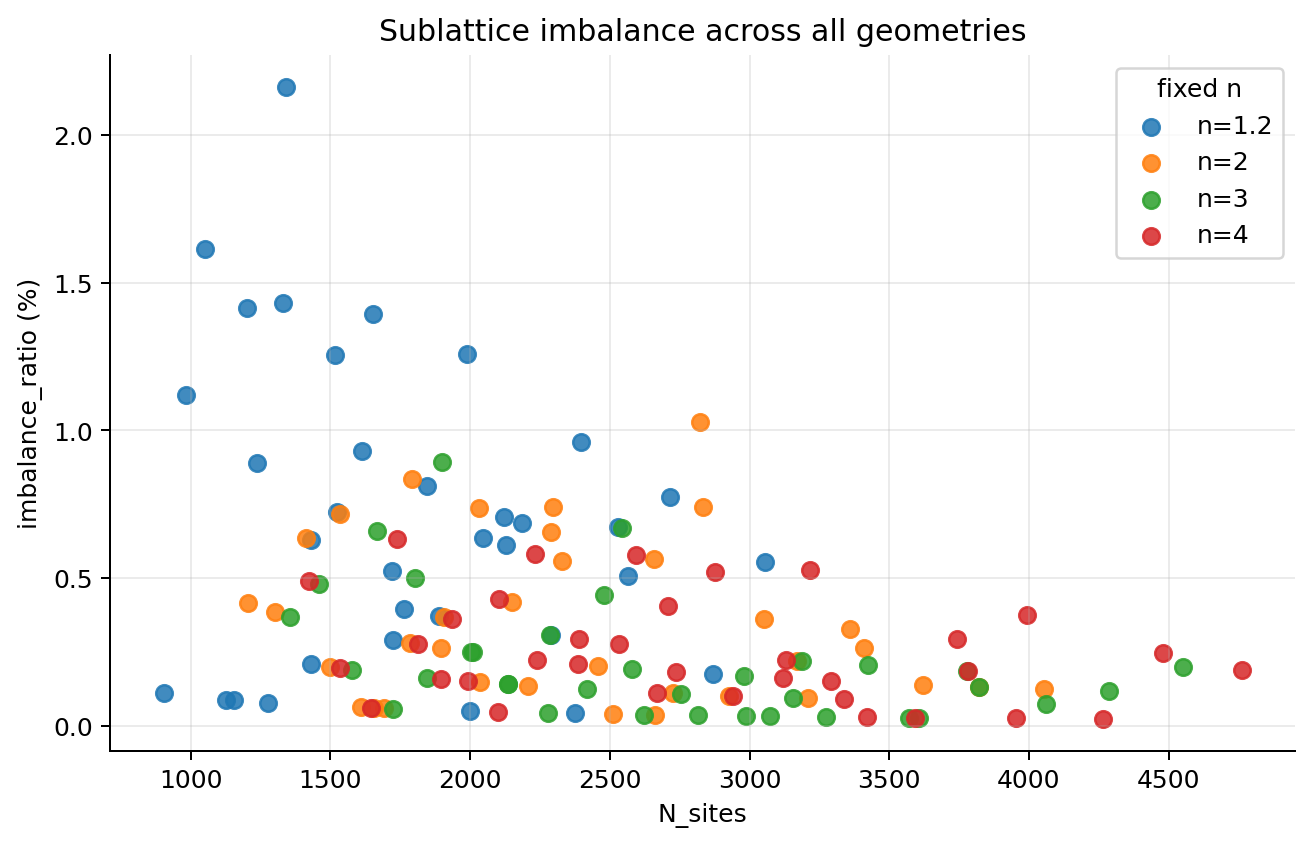
\includegraphics[width=0.85\textwidth]{../reports/assets/sublattice_imbalance_summary.png}
  \caption{TODO: Диагностика подрешёточного дисбаланса.}
\end{figure}

\section{Выводы по главе 3}
\todo{Сформулировать выводы: физический режим проверен, но это не доказательство continuum limit и не утверждение глобальной оптимальности признаков.}

\clearpage
